\section{Derivatives for example functions}

\begin{figure}[h]
		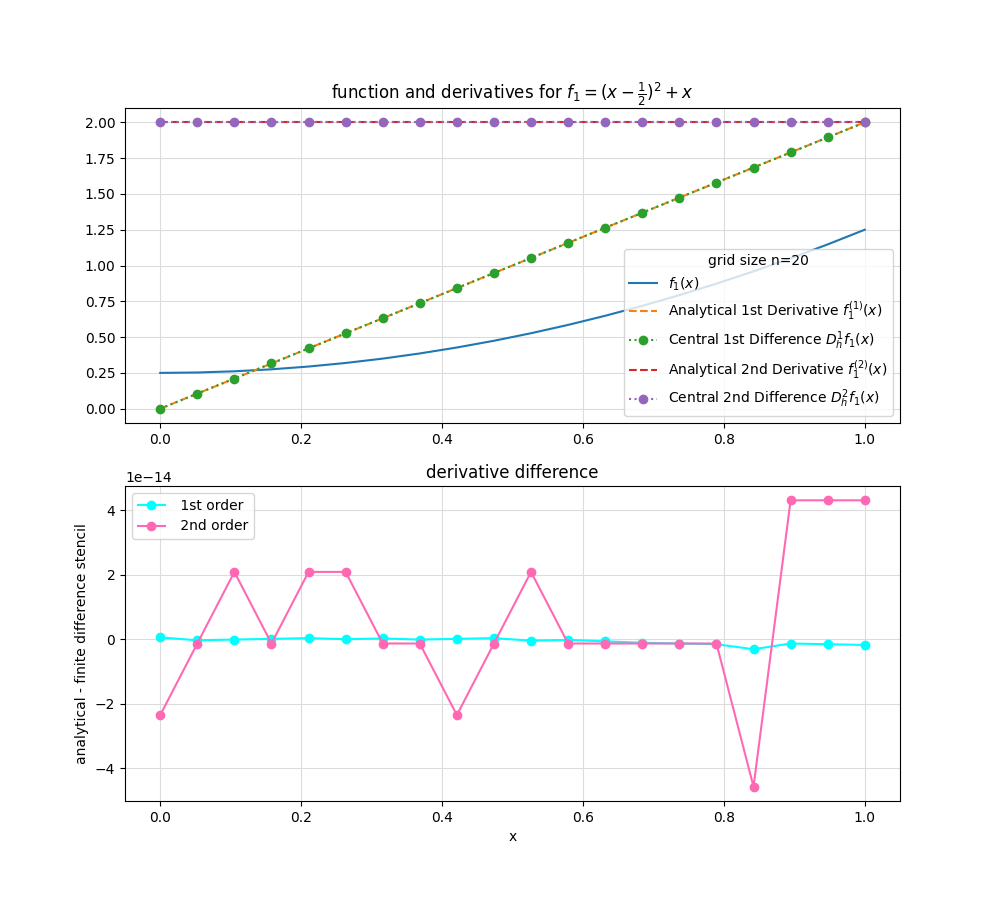
\includegraphics[scale=0.7]{plot_differences_analytical_finite_differences_f_1_n_20}
		\caption{Upper panel: Function $f_1$ in blue, dashed lines symbolize its analytical derivatives, dotted lines the finite difference approximation to the derivative. $n= 20$  Lower panel: The cyan and pink lines show the difference between analytical and numerically generated derivatives.
		One can see here, that for this quadratic function the error only consists of the roundoff error which stems from the finite computer storage}
\end{figure}

\begin{figure}
		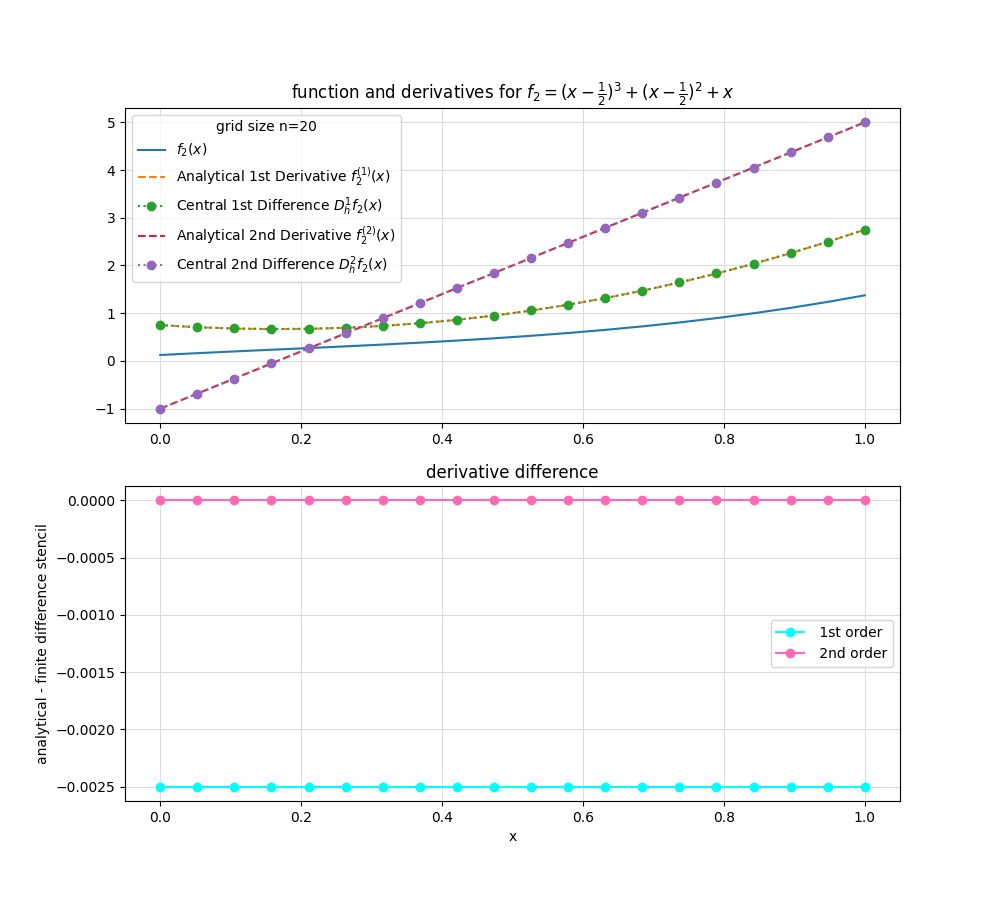
\includegraphics[scale=0.7]{plot_differences_analytical_finite_differences_f_2_n_20}
		\caption{ Here the error term for both differences is constant. As the function itself is of order 3, one now truely has a truncation error.}
\end{figure}

\begin{figure}
		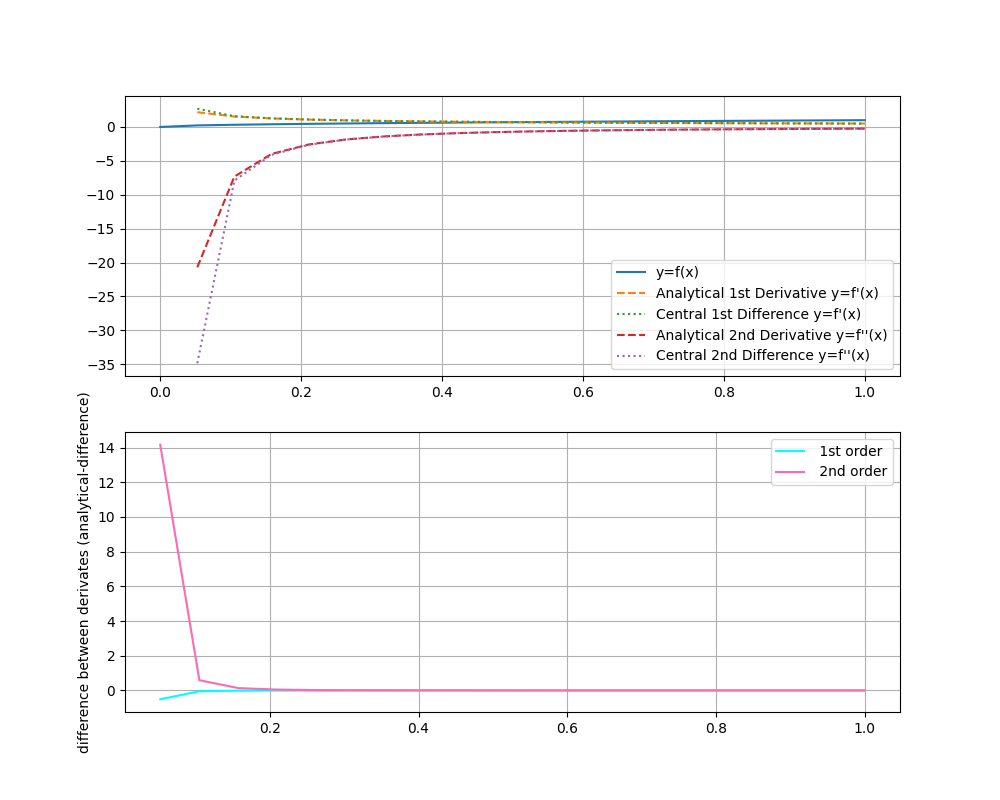
\includegraphics[scale=0.7]{plot_differences_analytical_finite_differences_f_3_n_20}
	\caption{Here the error term for both derivatives vanishes quickly. It stems from the fact, that one uses central difference stencils even though one doesn't have all the function values necessary (since one cannot take the squareroot of negative numbers}.
\end{figure}

\begin{figure}
		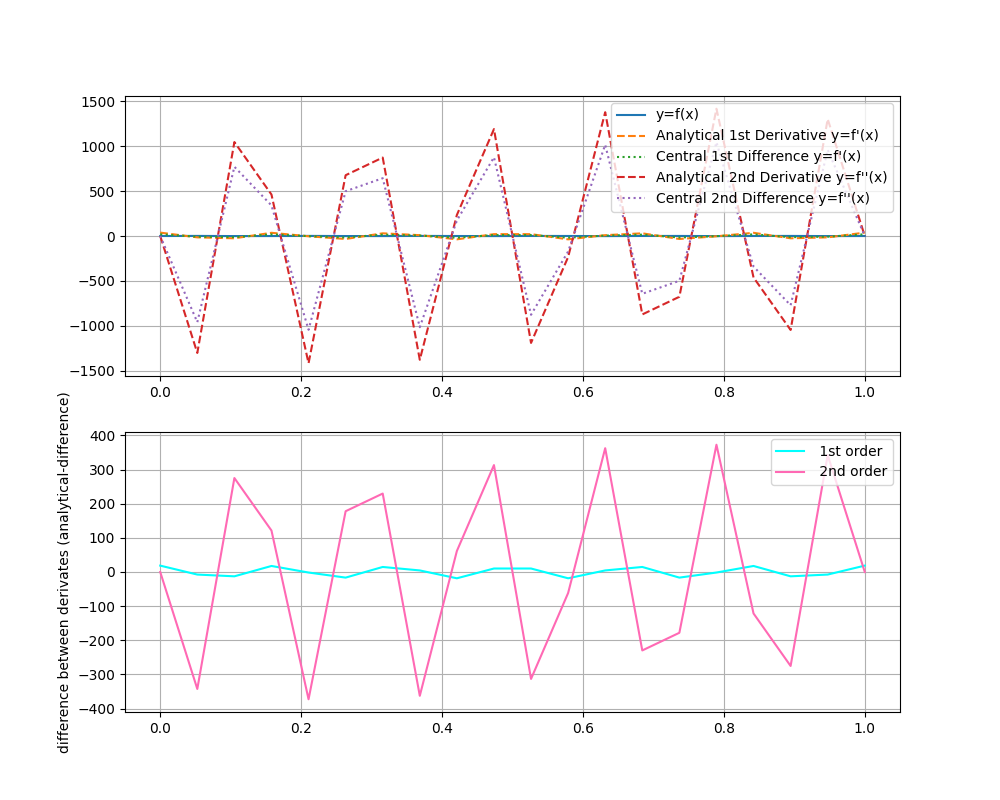
\includegraphics[scale=0.7]{plot_differences_analytical_finite_differences_f_4_n_20}
		\caption{}
\end{figure}


\begin{figure}
		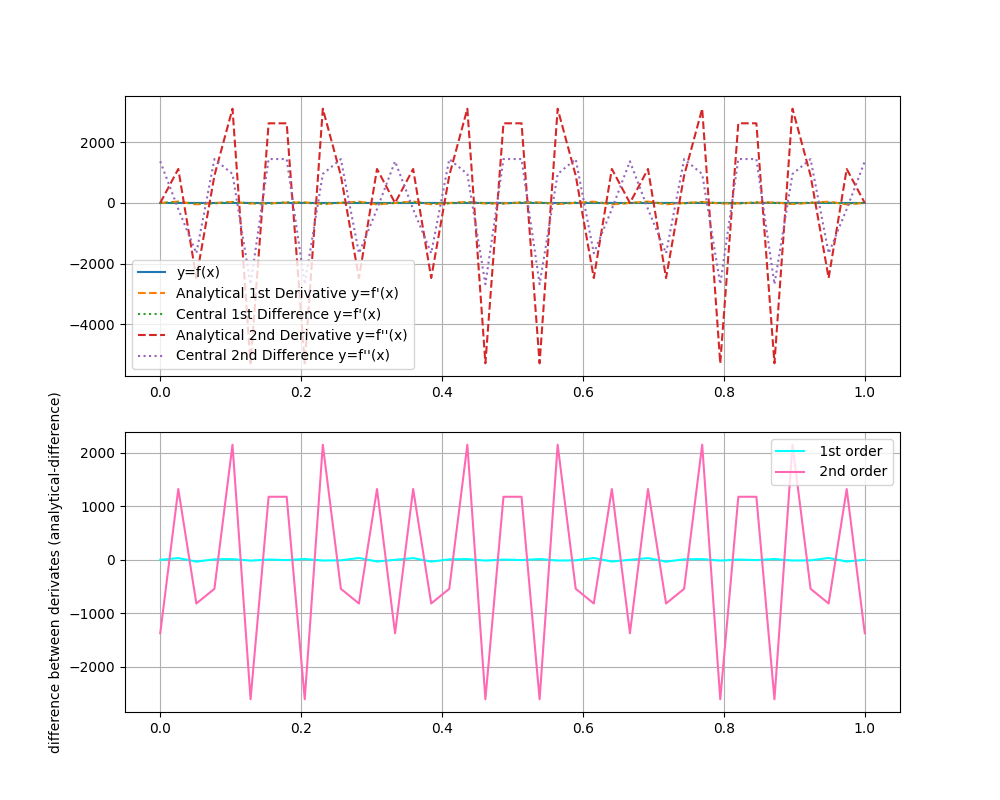
\includegraphics[scale=0.7]{plot_differences_analytical_finite_differences_f_5_n_40}
		\caption{}
\end{figure}


\begin{figure}
		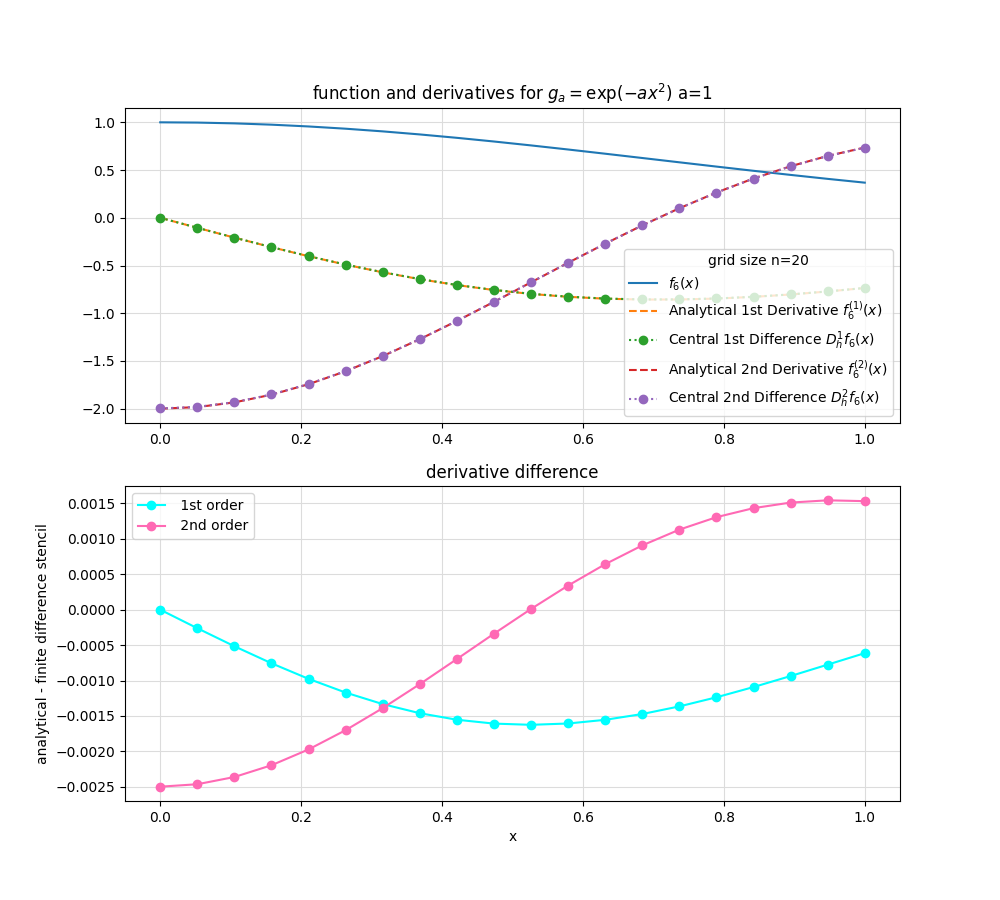
\includegraphics[scale=0.7]{plot_differences_analytical_finite_differences_f_a_n_20_a_1}
		\caption{}
\end{figure}

\begin{figure}
	\centering
	\begin{subfigure}[b]{\textwidth}
		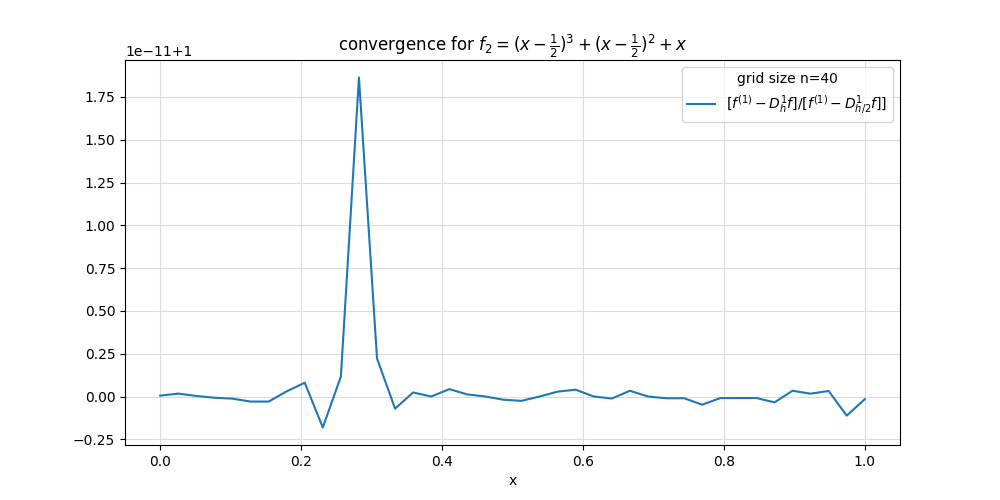
\includegraphics[width =\textwidth]{convergence_f_2_n_40}
		\caption{convergence}
	\end{subfigure}
	\hfill 
	\begin{subfigure}[b]{\textwidth}
		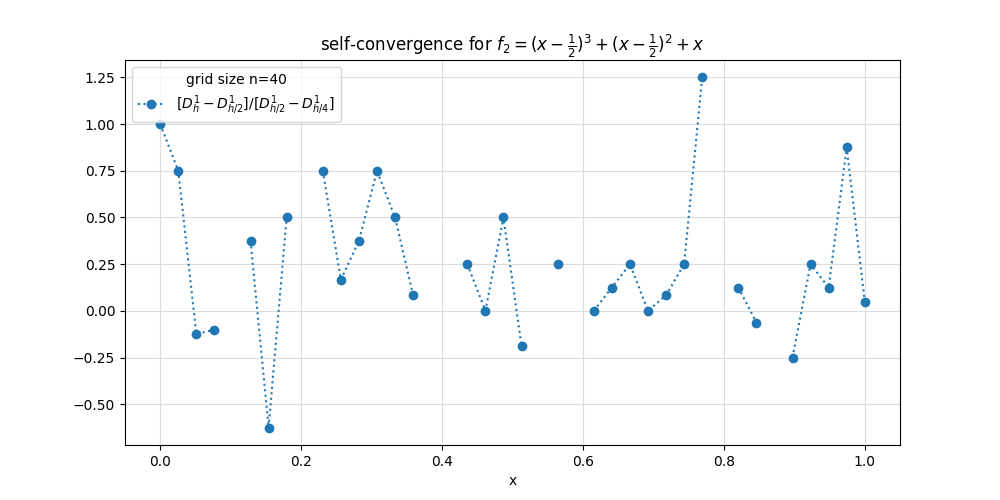
\includegraphics[scale=0.7]{self_convergence_f_2_n_40}
		\caption{self-convergence}
	\end{subfigure}
\end{figure}
\begin{figure}
		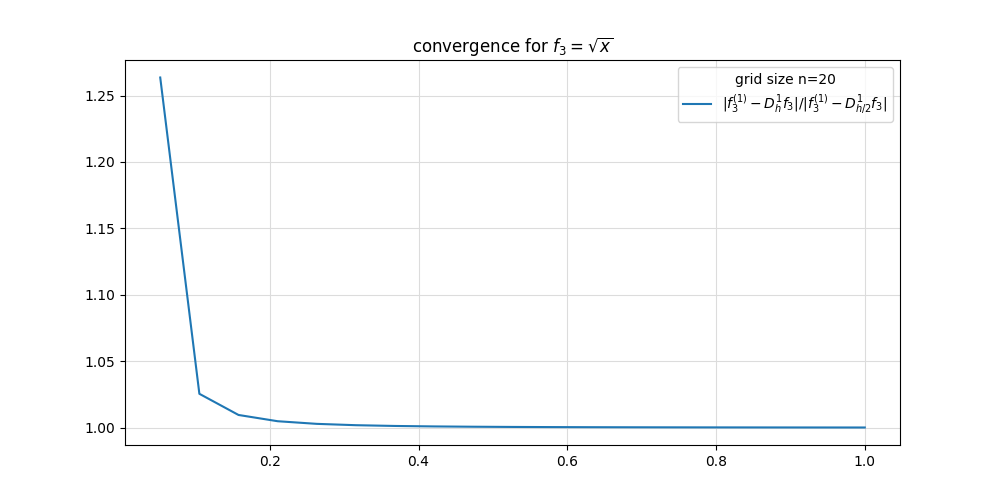
\includegraphics[scale=0.7]{convergence_f_3_n_20}
		\caption{ }
\end{figure}

\begin{figure}
		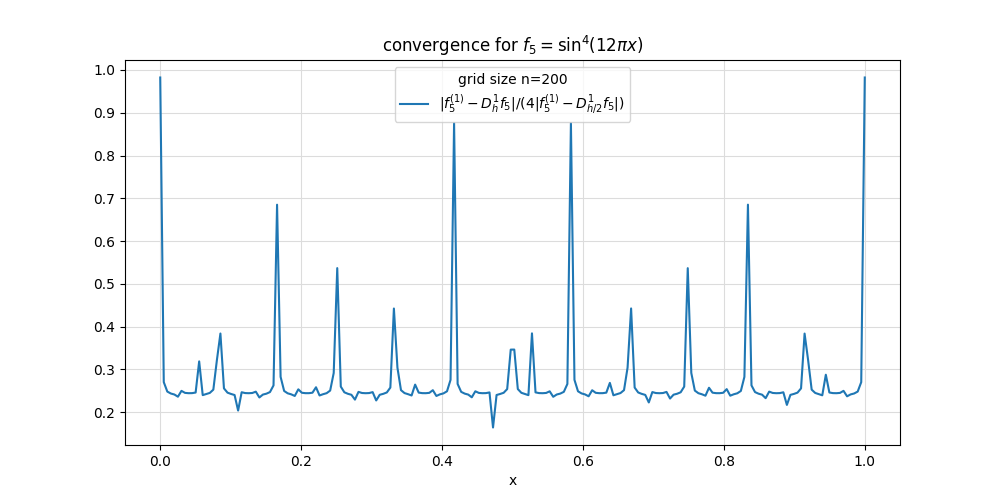
\includegraphics[scale=0.7]{modified_convergence_f_5_n_200}
		\caption{ convergence for function }
\end{figure}

\begin{figure}
		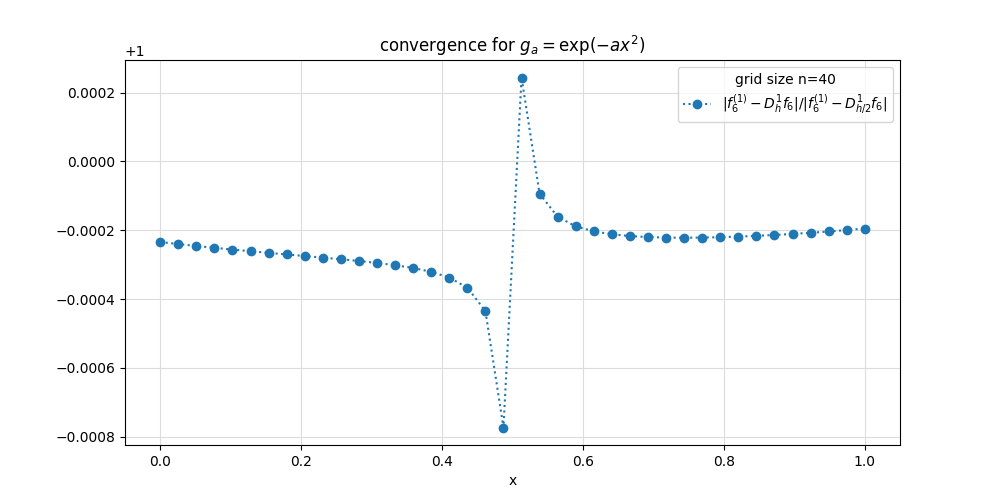
\includegraphics[scale=0.7]{convergence_f_6_n_40}
		\caption{ convergence for function }
\end{figure}
\newpage